\section{Fundamental Theorem of Calculus}
%=========================================================================
% Start of first day's activities
%=========================================================================
\preClass{Riemann Sums}

\begin{problem}
  \item Determine the value of the integral
  \begin{eqnarray*}
    \int^3_1 f(x) ~ dx,
  \end{eqnarray*}
  where the graph of the function, $f(x)$, is given below.

   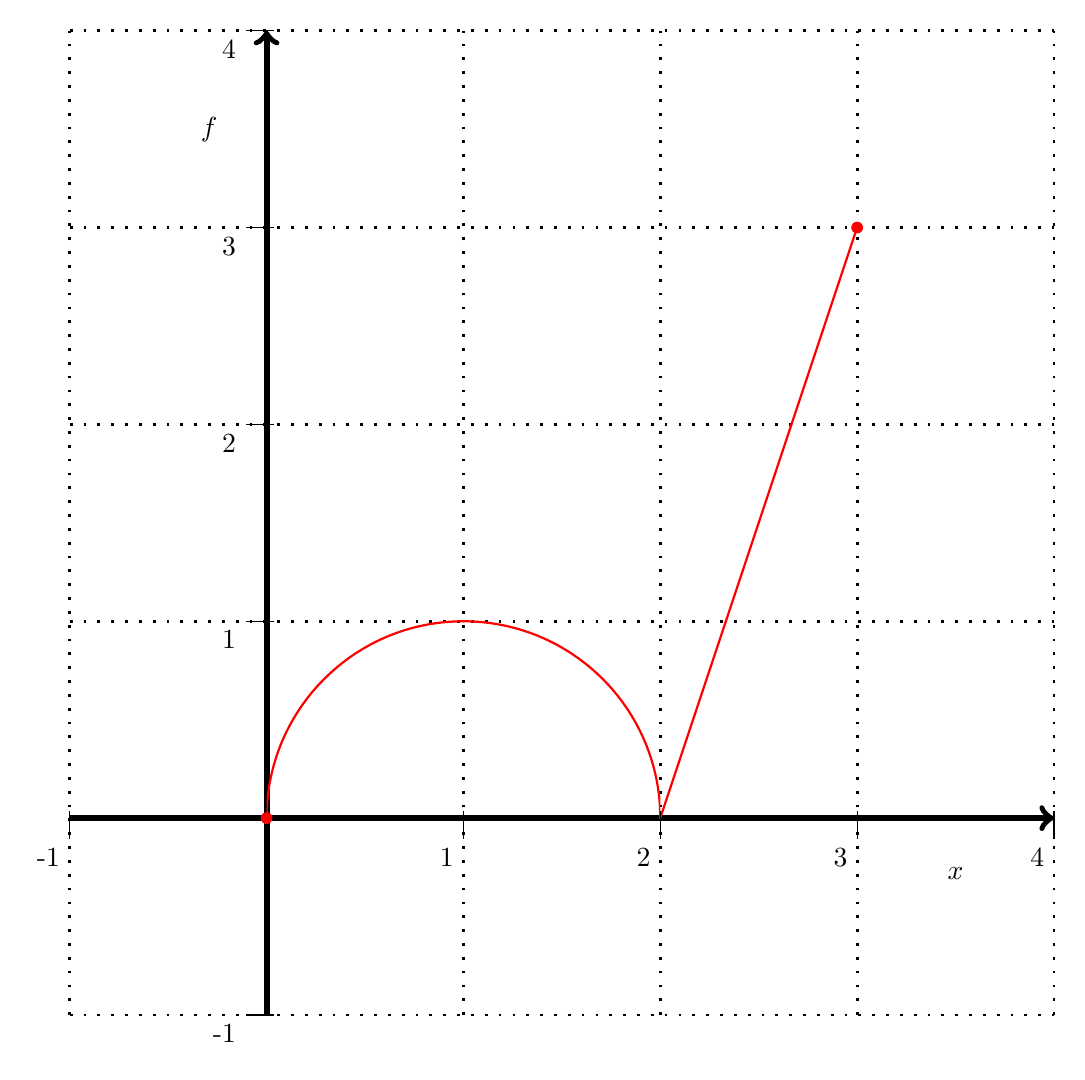
\begin{tikzpicture}[scale=2.5]
     \draw[step=1,loosely dotted,line width=1] (-1,-1) grid (4,4);
     \draw[line width=2.2,->] (-1,0) -- (4,0);
     \draw[line width=2.2,->] (0,-1) -- (0,4);
     \begin{scope}
       \clip (0,0) rectangle (2,2);
       \draw[red,thick] (1,0) circle(1.0);
     \end{scope}
     \draw[red,thick] (2,0) -- (3,3);
     \fill[red] (0,0) circle(0.03);
     \fill[red] (3,3) circle(0.03);
     \node[left] at (-0.2,3.5) {$f$};
     \node[below] at (3.5,-0.2) {$x$};
     \foreach \x in {-1,1,2,3,4}
        \draw (\x,1pt) -- (\x,-3pt) node[anchor=north east] {\x};
     \foreach \y in {-1,1,2,3,4}
         \draw (1pt,\y) -- (-3pt,\y) node[anchor=north east] {\y};
    \end{tikzpicture}

  \clearpage

  \item Approximate the integral
  \begin{eqnarray*}
    \int^3_1 \ln(x) ~ dx
  \end{eqnarray*}
  using a Riemann sum with 3 rectangles of equal width.

  \clearpage

\end{problem}


\actTitle{Riemann Sums}

\begin{problem}
\item A long, thing rod is five meters long and has a charge density given by
  \begin{eqnarray*}
    \lambda_q & = & 5x~\frac{\mathrm{C}}{\mathrm{m}},
  \end{eqnarray*}
  where $x$ is between 0m and 5m.
  \begin{subproblem}
  \item Make a rough sketch of the rod.
    \vspace{4em}
  \item Divide the rod into 5 equal parts, and determine the length of
    each part. Determine the coordinates for the endpoints of each part.
    \vfill
  \item Determine the charge density at the left endpoint of each part
    of the rod.
    \vfill
    \clearpage
  \item Determine an estimate for the total charge of each part
    assuming that the charge density is roughly constant over each
    part.
    \vfill
    \vfill
  \item Determine an estimate for the total charge in the rod.
    \vfill
    \vfill
    \clearpage
  \item Make a sketch of the charge density function.
    Include a geometric interpretation of the sum you found in the previous questions.
    \sideNote{Mark the heights you used in your sum and show how the widths relate geometrically in the sum.}
      \vfill
      \vfill
      \vfill
  \item How can you improve the estimate of the total charge?
    \vspace{2em}
  \item What is the relationship between your estimate of the total charge and the density function graphed above?
    \vfill
    \clearpage
  \item Determine the total charge in the rod.
    \vfill
  \end{subproblem}
\end{problem}

\postClass

\begin{problem}
\item Briefly state two ideas from today's class.
  \begin{itemize}
  \item
  \item
  \end{itemize}
\item
  \begin{subproblem}
    \item
  \end{subproblem}
\end{problem}



%=========================================================================
% Start of second day's activities
%=========================================================================
\preClass{Integrals}

\begin{problem}
  \item Determine the value of the following integrals.
    \begin{subproblem}
    \item $\int^5_0 2x ~ dx$
      \vfill
    \item $\int^5_0 2x^2 ~ dx$
      \vfill
    \item $\int^5_0 2x^2 - 2x ~ dx$
      \vfill
    \end{subproblem}
\end{problem}


\actTitle{Integrals}

\begin{problem}
\item A thin rod has a charge density given by
  \begin{eqnarray*}
    \lambda_q & = & x e^{-x^2}~\frac{\mathrm{C}}{\mathrm{m}},
  \end{eqnarray*}
  where $x$ is between 1m and 5m.
  \begin{subproblem}
  \item Make a rough sketch of the rod.
    \vspace{4em}
  \item Divide the rod into 5 equal parts, and determine the length of
    each part, and the coordinates for the endpoints.
    \vfill
  \item Determine the formula for the charge density on the left
    endpoint of each part from above.
    \sideNote{You can leave your answer as an expression and do not need to calculate the numerical values.}
    \vfill
  \item Use the charge densities above to approximate the total charge in the rod.
    \vfill
    \clearpage
 \item Make a rough sketch of the rod.
      \vspace{3em}
\item Divide the rod into $N$ equal parts, and determine the length of
      each part, and the coordinates for the endpoints.
      \sideNote{The expressions should depend on $N$.}
      \vfill
  \item Determine the sum using sigma notation for the estimate of the
    total charge in the rod.
    \vfill
  \item Express the limit of the sum as an integral.
    \vfill
  \item Determine the amount of charge in the rod.
    \vfill
  \item Make a sketch of the charge density function, and indicate the geometric relationship between the density and the total charge.
    \vfill
  \end{subproblem}
  \clearpage
  \item The function $h$ is defined by
  \begin{eqnarray*}
    h(x) & = & \sin(x).
  \end{eqnarray*}
  The function $g$ satisfies $g(0)=0$ and $g(1)=\frac{\pi}{2}$.
  Determine the value of the integral
  \begin{eqnarray*}
    \int^1_0 h(g(x)) g'(x) ~ dx.
  \end{eqnarray*}
  \vfill

  \clearpage

  \item The function $H$ satisfies $H(0)=5$ and $H(1)=10$.
  Determine the value of the integral
  \begin{eqnarray*}
    \int^{\frac{\pi}{2}}_0 H'(\cos(x)) \sin(x) ~ dx.
  \end{eqnarray*}
  \vfill
\end{problem}


\postClass

\begin{problem}
\item Briefly state two ideas from today's class.
  \begin{itemize}
  \item
  \item
  \end{itemize}
  \item Determine the values of each of the following integrals.
    \begin{subproblem}
    \item $\int^{10}_1 \frac{1}{1+x^2} ~ dx$
      \vfill
    \item $\int^{10}_1 \frac{x}{1+x^2} ~ dx$
      \vfill
    \item $\int^{10}_1 \frac{e^x}{1+e^{x}} ~ dx$
      \vfill
    \end{subproblem}
  \item A long, thin rod has a charge distribution, and the length of the rod is
      2m. The left endpoint is $x=0$m, and the right endpoint is
      $x=2$m. Determine the total charge in the rod for the following
      charge densities.
      \begin{subproblem}
        \item $\lambda_q = \frac{e^x}{1+e^{2x}}$ C/m
          \vfill
        \item $\lambda_q = x\sin\lp 1+x^2\rp$ C/m
          \vfill
      \end{subproblem}
\end{problem}


%=========================================================================
% Dedicated day to practice with u-substitution
%=========================================================================
\preClass{Integrals}

\begin{problem}
  \item Determine the value of the following integrals.
    \begin{subproblem}
    \item ${\displaystyle \int^\pi_0 x \sin\left(3x^2\right) ~  dx}$
      \vfill
    \item ${\displaystyle \int^1_0  \sqrt{1-x^2} ~ dx}$
      \vfill
    \item ${\displaystyle \int^5_0 x \sqrt{1-x^2} ~ dx }$
      \vfill
    \end{subproblem}
\end{problem}


\actTitle{Integrals}

\begin{problem}
\item For the following questions assume that $f(t)$ and $g(t)$ are continuous and differentiable functions.
  \begin{subproblem}
  \item Determine another expression for the derivative
    \begin{eqnarray*}
        \frac{d}{dt} f(g(t)).
    \end{eqnarray*}
    \vfill
  \item Determine the value of
  \begin{eqnarray*}
    \int^1_0 \frac{d}{dt} f(g(t)) ~ dt.
  \end{eqnarray*}
    \vfill
  \item What does this result imply about the value of
    \begin{eqnarray*}
      \int^1_0 f'(g(t))g'(t) ~ dt?
    \end{eqnarray*}
    \vfill
  \end{subproblem}

    \clearpage
 \item 
\item
      \vfill
  \item
    \vfill

  \clearpage
  \item

  \clearpage

  \item
  \vfill
\end{problem}


\postClass

\begin{problem}
\item Briefly state two ideas from today's class.
  \begin{itemize}
  \item
  \item
  \end{itemize}
  \item ~
    \begin{subproblem}
    \item ~
      \vfill
    \item ~
      \vfill
    \item ~
      \vfill
    \end{subproblem}
\end{problem}


%=========================================================================
% First day of int. by parts
%=========================================================================
\preClass{Integraton}

\begin{problem}
  \item We examine the product rule.
  \begin{subproblem}
    \item   State the product rule for the function below:
  \begin{eqnarray*}
    \lefteqn{\frac{d}{dt} \lp f(t) g(t) \rp  ~ = } \hspace{20em} \\
    & &
  \end{eqnarray*}
  \item Use the product rule to expand the derivative of $h(t)=g(t)e^t$ in terms of
      $g$ and $g'$:
      \begin{eqnarray*}
        \frac{d}{dt} h(t) & = &  \frac{d}{dt} \lp g(t) e^t \rp
      \end{eqnarray*}
      \vfill
  \item   Solve the previous equation for $g(t) \cdot e^t$.
  \vfill
\end{subproblem}
\end{problem}



\actTitle{Integration by Parts}
\begin{problem}
\item A rod has a charge distribution, and the length of the rod is
  3m. The left endpoint is $x=0$m, and the right endpoint is
  $x=3$m. Determine the total charge in the rod for the following
  charge densities.
  \begin{subproblem}
    \item $\lambda_q = xe^{4x}$ C/m
      \vfill
    \item $\lambda_q = 3+x\sin(5x)$ C/m
      \vfill
      \clearpage
    \item $\lambda_q = x^2 e^{2x} $ C/m
      \vfill
  \end{subproblem}
  \item  Determine the value of the integral
  \begin{eqnarray*}
    \int_{x=0}^\infty x e^{-sx} ~ dx,
  \end{eqnarray*}
  where $s>0$. (Treat $s$ as if it is were a constant.)
  This integral is a function of a variable. What variable is it a function of?
  \vfill
  \clearpage
  \item Determine the value of the integral
  \begin{eqnarray*}
    \int^{10}_1 \ln(x) ~ dx.
  \end{eqnarray*}
  (Hint: express $\ln(x)=1\cdot\ln(x)$ and use the two functions, $1$ and $\ln(x)$, when integrating by parts.)
\end{problem}

\postClass

\begin{problem}
\item Briefly state two ideas from today's class.
  \begin{itemize}
  \item
  \item
  \end{itemize}
\item
  \begin{subproblem}
    \item
  \end{subproblem}
\end{problem}


%=========================================================================
% First day of int. by parts / Day II
%=========================================================================
\preClass{Integraton}

\begin{problem}
\item Determine the values of each of the following integrals.
  \begin{subproblem}
  \item $\int^{3}_1 x e^{-x} ~ dx$
    \vfill
  \item $\int^{3\pi}_1 x^2 e^{2x} ~ dx$
    \vfill
  \end{subproblem}
\end{problem}



\actTitle{Integration by Parts}
\begin{problem}
\item A rod has a charge distribution, and the length of the rod is
  3m. The left endpoint is $x=1$m, and the right endpoint is
  $x=3$m. Determine the total charge in the rod for the following
  charge densities.
  \begin{subproblem}
    \item $\lambda_q = \frac{\ln(x)}{x^2} $ C/m
      \vfill
    \item $\lambda_q = e^{\sqrt{x}}$ C/m
      \vfill
  \end{subproblem}
  \clearpage
  \item  Determine the value of the integral
  \begin{eqnarray*}
    \int_{x=0}^\infty \cos(x) e^{-sx} ~ dx.
  \end{eqnarray*}
  Treat $s$ as if it were a constant parameter. What are the possible values of $s$?
  \vfill
  \clearpage
  \item On the previous question what are the possible pitfalls of using integration by parts?
  What are the general guidelines you have to use to solve the problem?
    \vspace{6em}

  \item Suppose that a function, $f(x)$, is increasing on an interval from $x=a$ to $x=b$ ($a<b$).
  Another function, $g$, is positive on the same interval and $g(a)=g(b)=0$. Show that
  \begin{eqnarray*}
    \int^b_a f(x) g'(x) ~ dx & \leq & 0.
  \end{eqnarray*}
  How do you interpret the meaning of this result?

  \vfill

\end{problem}

\postClass

\begin{problem}
\item Briefly state two ideas from today's class.
  \begin{itemize}
  \item
  \item
  \end{itemize}
\item The questions below refer to the integral
\begin{eqnarray*}
  \int^M_0 f'(x) e^{-sx} ~ dx,
\end{eqnarray*}
where $s>0$.
  \begin{subproblem}
    \item Use integration by parts to change the integral into an integral
    that has $f(x)$ and not its derivative.
     \vfill
     \item Simplify the expression by assuming that $f(M)e^{-sM}$ goes to zero as $M\rightarrow\infty$.
     \
  \end{subproblem}
  \item Determine the value of the integral
    \begin{eqnarray*}
      \int_{x=0}^\infty \sin(\omega x) e^{-sx} ~ dx.
    \end{eqnarray*}
    Treat $\omega$ and $s$ as constant parameters. What are the limitations on $s$?

\end{problem}


%=========================================================================
% Trig substitutions
%=========================================================================
\preClass{Integraton}

\begin{problem}
\item For each of the triangles below, determine the length of the
  side with the missing length. Also, determine the sine, cosine, and tangent
  for the angle in the lower right part of the triangle.
  \begin{subproblem}
  \item 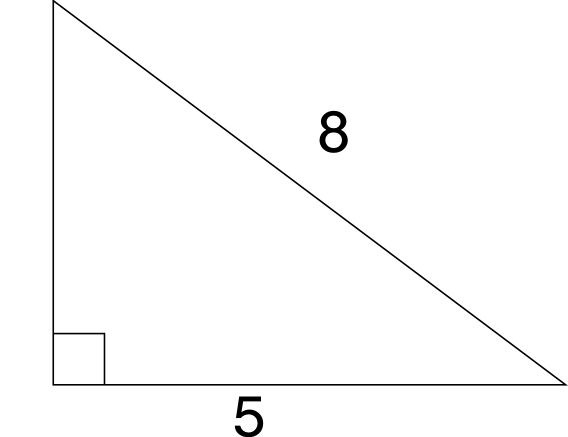
\includegraphics[width=10em]{ink/trigSubs/triangleValuesBottomHyp}
    \vfill
  \item 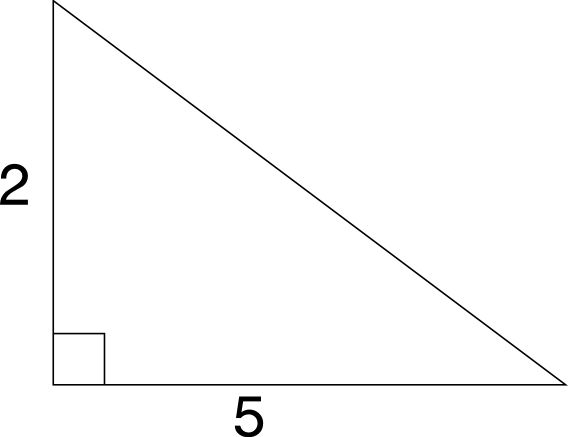
\includegraphics[width=10em]{ink/trigSubs/triangleValuesLeftBottom}
    \vfill
  \item 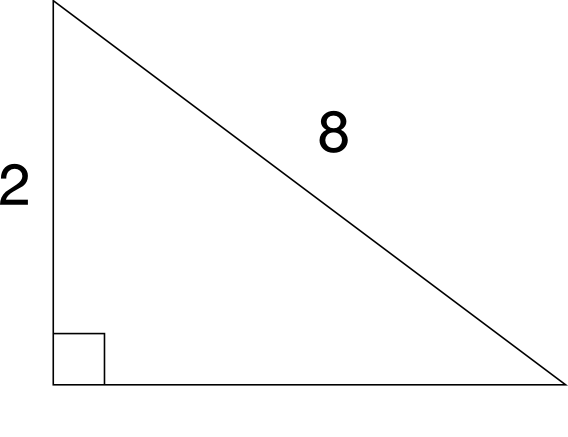
\includegraphics[width=10em]{ink/trigSubs/triangleValuesLeftHyp}
    \vfill
  \end{subproblem}
\end{problem}



\actTitle{Trigonometric Substitution}
\begin{problem}
  \item  A rod of length 2m has a uniform charge density, $\lambda_q$ C/m.
  The center of the rod is placed at the origin and is aligned along the
  $x$-axis.
  \begin{subproblem}
    \item Make a rough sketch of the rod.
         \vspace{5em}
   \item Divide the rod into $n$ equal parts, and determine the length of
         each part, and the coordinates for the endpoints.
         \vspace{2em}
     \item Mark a point 1m above the center of the rod in your picture. Determine the
         electric field due to the charge in one small piece of the rod.
         (Determine the $\vec{i}$ and $\vec{j}$ components separately.)
       \vfill
     \item Add up the components of the electic field to get a sum representing the
      $\vec{i}$ and $\vec{j}$ components of the electic field.
      \vfill
    \clearpage
    \item Determine the integrals that represent the $\vec{i}$ and $\vec{j}$ components of the electic field.
      Determine the values of the integrals and determine the electric field above the center of the rod.
      \vfill
  \end{subproblem}

\end{problem}

\postClass

\begin{problem}
\item Briefly state two ideas from today's class.
  \begin{itemize}
  \item
  \item
  \end{itemize}
  \item A rod has a charge distribution.
    The left endpoint is $x=0$m, and the right endpoint is
    $x=0.5$m. Determine the total charge in the rod for the following
    charge densities.
    \begin{subproblem}
      \item $\lambda_q = \frac{1}{\sqrt{1-x^2}}$ C/m
        \vfill
      \item $\lambda_q = \frac{1}{\sqrt{4-x^2}}$ C/m
        \vfill
    \end{subproblem}
  \item  A rod of length 4m has a uniform charge density, $\lambda_q$ C/m.
    The center of the rod is placed at the origin and is aligned along the
    $x$-axis.
    \begin{subproblem}
      \item Determine the electric field 1m above the center of the rod.
      \item Determine the electric field $l$m above the center of the rod,
        where $l$ is a constant.
      \item Determine the electric field at any point above the rod.
    \end{subproblem}

  \item  A rod of infinite length has a uniform charge density, $\lambda_q$ C/m.
      \begin{subproblem}
        \item Determine the electric field 1m above the rod.
        \item Determine the electric field $l$m above the rod,
          where $l$ is a constant.
        \item Determine the electric field at any point above the rod.
      \end{subproblem}


\end{problem}


%=========================================================================
% Trig substitutions - day 2
%=========================================================================
\preClass{Integraton}

\begin{problem}
\item For each of the triangles below, determine the length of the
  side with the missing length. Also, determine the sine, cosine, and tangent
    for the angle in the lower right part of the triangle.
  \begin{subproblem}
  \item 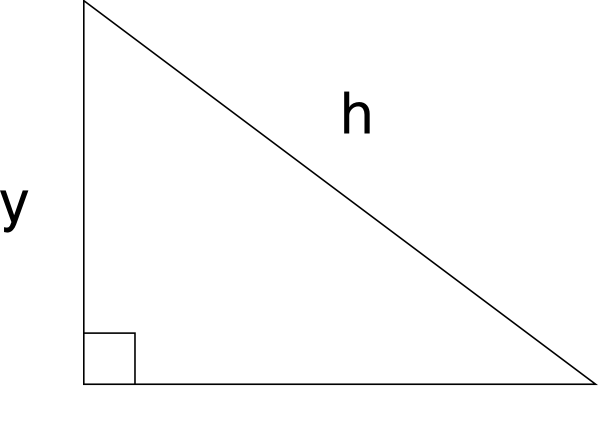
\includegraphics[width=10em]{ink/trigSubs/triangleSymbolsLeftHyp}
    \vfill
  \item 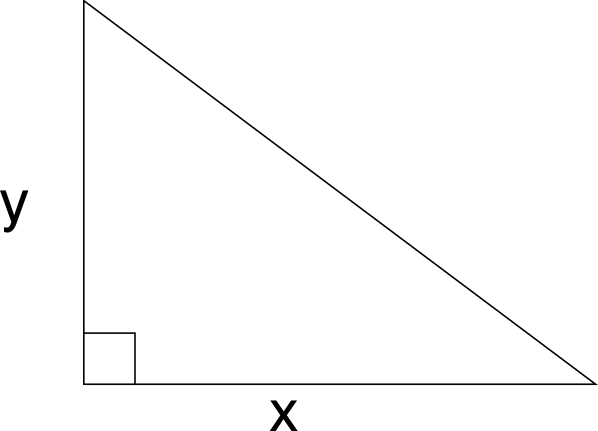
\includegraphics[width=10em]{ink/trigSubs/triangleSymbolsBottomLeft}
    \vfill
  \item 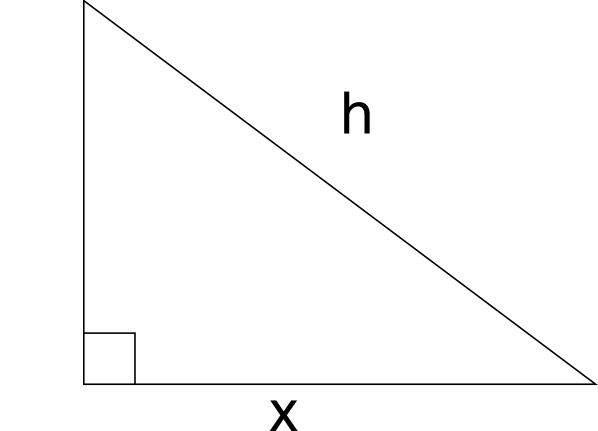
\includegraphics[width=10em]{ink/trigSubs/triangleSymbolsBottomHyp}
    \vfill
  \end{subproblem}
\end{problem}



\actTitle{Trigonometric Substitution}
\begin{problem}
  \item  A rod of length 4m has a uniform charge density, $\lambda_q$ C/m.
  The center of the rod is placed at the origin and is aligned along the
  $x$-axis.
  \begin{subproblem}
    \item Make a rough sketch of the rod.
         \vspace{5em}
   \item Divide the rod into $n$ equal parts, and determine the length of
         each part, and the coordinates for the endpoints.
         \vspace{2em}
     \item Mark a point 3m above the \textbf{right end} of the rod in your picture. Determine the
         electric field due to the charge in one small piece of the rod.
         (Determine the $\vec{i}$ and $\vec{j}$ components separately.)
       \vfill
     \item Add up the components of the electic field to get a sum representing the
      $\vec{i}$ and $\vec{j}$ components of the electic field.
      \vfill
    \clearpage
    \item Determine the integrals that represent the $\vec{i}$ and $\vec{j}$ components of the electic field at the point.
      Determine the values of the integrals and determine the electric field above the center of the rod.
      \vfill
  \end{subproblem}

\clearpage

\item A rod has a charge distribution, and the length of the rod is
  3m. The left endpoint is $x=0$m, and the right endpoint is
  $x=3$m. Determine the total charge in the rod for the following
  charge densities.
  \begin{subproblem}
    \item $\lambda_q = \frac{x}{\sqrt{9-x^2}}$ C/m
      \vfill
    \item $\lambda_q = \frac{x^2}{\sqrt{x^2-9}}$ C/m
      \vfill
  \end{subproblem}
\end{problem}

\postClass

\begin{problem}
\item Briefly state two ideas from today's class.
  \begin{itemize}
  \item
  \item
  \end{itemize}
\item A rod of length $l$ has a uniform charge density, $\lambda_q$ C/m,
    and the right side of the rod is located at the origin.
    \begin{subproblem}
      \item Determine the electric field $y$m above the right side of the rod,
        where $y$ is a constant.
      \item Determine what happens as the length $l$ gets extremely long.
        Does the electric field approach a particular value?
    \end{subproblem}
\item A rod has a charge distribution, and the length of the rod is
  2m. The left endpoint is $x=1$m, and the right endpoint is
  $x=1$m. Determine the total charge in the rod for the following
  charge densities.
  \begin{subproblem}
    \item $\lambda_q = \frac{x}{\sqrt{1+x^2}}$ C/m
      \vfill
    \item $\lambda_q = \frac{x^3}{\sqrt{4+x^2}}$ C/m
      \vfill
  \end{subproblem}
\end{problem}


%=========================================================================
% E-Field for a ring
%=========================================================================
\preClass{Arc-length of a circle.}

\begin{problem}
\item A person moves around a circle of radius 10m. Answer each of the questions below.
  \begin{subproblem}
  \item If the person moves around the whole circle how far has she traveled?
    \vfill
  \item If the person moves half way around the circle, through an angle of $\pi$, how far has she traveled?
    \vfill
  \item If the person moves around the circle through an angle of $\frac{\pi}{4}$ how far has she traveled?
    \vfill
  \item In general, if a person moves around a circle of radius $r$ through an angle $\theta$ how far has she traveled?
      \vfill
  \end{subproblem}
\end{problem}



\actTitle{Electric Field in Three Dimensions}
\begin{problem}
  \item  A thin, circular piece of metal has a uniform charge. The center of the circle is the origin,
        and it lies in the $x-y$ plane. The goal is to determine the electric field at a point above the
        center of the circle. The ring has a uniform charge, $\lambda_q$ C/m. \\
        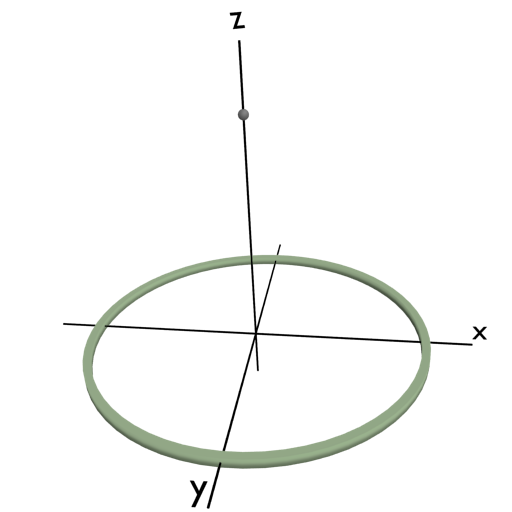
\includegraphics[width=15em]{blender/ringCharge}
  \begin{subproblem}
    \item Which direction do you think the electric field will point at the point above the circle? Why?
             \vspace{3em}
   \item The idea is to divide the ring into small pieces. Determine the charge in a small piece of the ring
       assuming that the length of the small piece is $\triangle s$. \\
           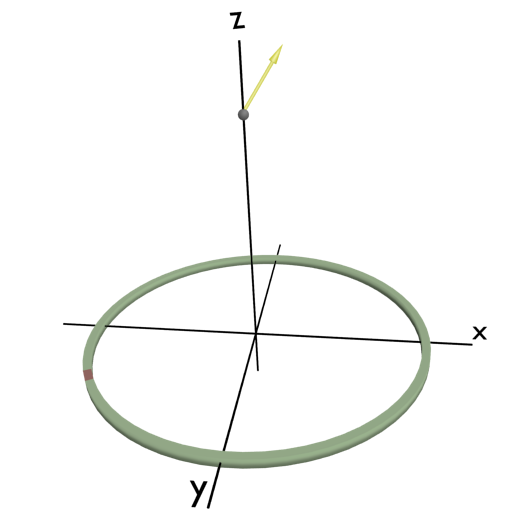
\includegraphics[width=10em]{blender/ringCharge-deltaE}

    \item If the point above the ring is a distance $l$ m over the origin and the radius of the circle is $R$,
      determine the magnitude of the electric field for the small piece. \\
        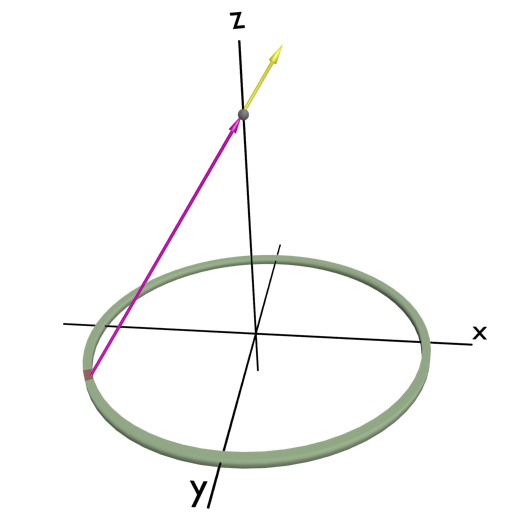
\includegraphics[width=10em]{blender/ringCharge-distance}

    \clearpage

     \item The electric field has three dimensions, components in the $\vec{i}$, $\vec{j}$, and $\vec{k}$ directions.
        The point above the ring is $l$ m above the center of the ring.
       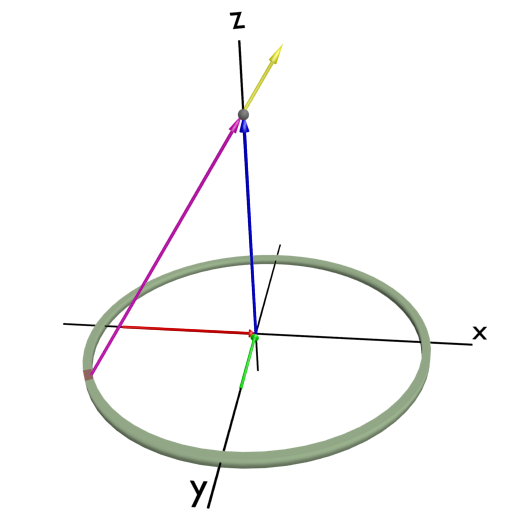
\includegraphics[width=15em]{blender/ringCharge-components}
       \begin{enumerate}
         \item Determine the component of $\triangle \vec{E}$ in the $z$-direction. (Hint: draw a side view of the triangle.)
         \vfill
         \item Determine the component of $\triangle \vec{E}$ pointing in the direction from the small piece towards the origin in the $x-y$ plane.
         \vfill
         \item Determine the component of $\triangle \vec{E}$ in the $x$-direction in terms of $\theta$.
         \vfill
         \item Determine the component of $\triangle \vec{E}$ in the $y$-direction in terms of $\theta$.
         \vfill
       \end{enumerate}
       \clearpage
     \item Determine the length of the small piece of charge in terms of $r$ and $\triangle\theta$.
         \vspace{2em}
     \item Add up the components of the electic field to get a sum representing the
      $\vec{\imath}$, $\vec{\jmath}$, and $\vec{k}$ components of the electic field.
      \vfill
    \item  Determine the Riemann sum that approximates the $\vec{\imath}$, $\vec{\jmath}$, and $\vec{k}$ components of the electic field at the point.
      \vspace{4em}
    \item Determine the integrals that represent the $\vec{\imath}$, $\vec{\jmath}$, and $\vec{k}$ components of the electic field at the point.
      Determine the values of the integrals and determine the electric field above the center of the rod.
      \vfill
      \vfill
      \vfill
  \end{subproblem}

\end{problem}

\postClass

\begin{problem}
\item Briefly state two ideas from today's class.
  \begin{itemize}
  \item
  \item
  \end{itemize}
\end{problem}

%=========================================================================
% E-Field for a plate
%=========================================================================
\preClass{Electric field for a ring}

\begin{problem}
\item Use the results from the previous activity.
  \begin{subproblem}
  \item What is the electric field for a point $l$ meters above the center of a thin ring of radius $r$ above the ring?
    The charge density on the ring is a constant, $\lambda_q$ C/m.
    \vfill
  \item What is the area of a circle of radius $r$?
    \vfill
  \item What is the area of a circle of radius $r+\triangle r$?
      \vfill
  \item What is the area between a circle of radius $r$ and a circle of radius $r+\triangle r$?
    \sideNote{Foil out the value and simplify it as much as possible.}
      \vfill
  \end{subproblem}
\end{problem}



\actTitle{Electric Field Over a Circular Plate}
\begin{problem}
  \item The goal is to derive the function that represents the electric field over the center of
    a thin circular plate with radius $R$ and a constant charge density $\sigma_q$ C/m\textsuperscript{2}.
    Refer to the previous day's activities and repeat the steps on your own.
  \begin{subproblem}
    \item Draw a picture of the plate with a point $l$ meters above the center of the plate.
      \vfill
   \item Divide the plate into thin rings each with width $\triangle r$.  (Redraw the picture.)
      \vfill
   \item Determine the electric field for one of the thin rings.  (Redraw the picture.)
       \vfill

    \clearpage

   \item Determine the domain of the function representing the electric field, $\triangle \vec{E}$
      for the small ring. (What variable is changing for the different rings?)
      \vspace{2em}

    \item Determine the Riemann sum for the electric field at the point above the ring.
      \vfill

    \item Determine the integral and solve the intregal that represents the electric field at the point above the ring.
      \vfill
      \vfill
      \vfill

    \clearpage

    \item Is the result consistent with the physical situation? Does it make sense?
       \vfill

     \item What happens as the radius of the disk increases?
        \vfill

      \item What happens as the distance above the disk increases?
       \vfill

  \end{subproblem}
\end{problem}

\postClass

\begin{problem}
\item Briefly state two ideas from today's class.
  \begin{itemize}
  \item
  \item
  \end{itemize}
\end{problem}

%=========================================================================
% Start of Volumes of Revolution
%=========================================================================
\preClass{Volumes of Revolution}

\begin{problem}
  \item What is the volume of a right circular cylinder that has a radius of $R$ and a height $h$?

    \vspace{3em}

  \item What is the volume of two cylinders stacked one on top of the other?
    The first is a right circular cylinder that has a radius of $R_1$ and a height $h_1$,
    and the second is a right circular cylinder that has a radius of $R_2$ and a height
    $h_2$.

    \vspace{3em}

\item Determine the value of the integral
  \begin{eqnarray*}
    \int^h_0 \pi \left (R-\frac{R}{h} x\right)^2 ~ dx,
  \end{eqnarray*}
  where $h$ and $R$ are constants.
  \vfill

\end{problem}


\actTitle{Volumes of Revolution}
\begin{problem}
\item Determine the formula for the volume of a cone.
    The base of the cone will have a radius of $R$ and the height will be $h$.
    The first step is to determine the formula for a line to revolve around the $x$ axis.
  \begin{subproblem}
    \item
      Make a sketch of the line that will be revolved around the $x$-axis.
      The base of the cone will be on the left ($x=0$), and the radius of the resulting cone should be $R$.
      The height will be along the $x$-axis and should have a length of $h$.
      (Sketch the axes and clearly annotate the axes.)
      \vfill

    \item Make a sketch of the resulting solid obtained after
      revolving the line around the $x$-axis.
      \vfill

    \item Break up the domain ($x$) into pieces. Each piece of the domain will be used to make a rectangle
         from the $x$-axis to the function. The rectangle will be rotated around the $x$-axis to form a small cylinder.
         Make a sketch of your function with one of the pieces revolved around the axis.
      \vfill

    \clearpage

    \item Determine the formula for the volume of one small cylinder at $x_i$. Your answer should only be a function of $x_i$.
      \vfill

    \item Determine the formula for the Riemann sum representing an approximation of the volume.
      \vfill

    \item Take an appropriate limit of the Riemann sum and express the sum as an integral.
      \vfill

    \item Evaluate the integral to get the volume of the cone.
      \vfill

  \end{subproblem}

  \clearpage

  \item A cone is formed by rotating a straight line around the $x$-axis.
     The cone has a charge density, and the charge is a function of $x$,
     \begin{eqnarray*}
       \lambda_C(x) & = & \frac{2}{x^2+3x+2} ~ \mathrm{C/m}^3
     \end{eqnarray*}
     The radius of the base of the cone is 0.3m, and the height of the cone is 0.4m.
     \begin{subproblem}
       \item
         Make a sketch of the line that will be revolved around the $x$-axis.
         The base of the cone will be on the left ($x=0$).
         The height will be along the $x$-axis.
         (Make an axis and clear mark the axes.)
         \vfill

       \item Make a sketch of the resulting solid obtained after
         revolving the line around the $x$ axis.
         \vfill

       \item Break up the domain ($x$) into pieces. Each piece of the domain will be used to make a rectangle
            from the $x$-axis to the function. The rectangle will be rotated around the $x$ axis to form a small cylinder.
            Make a sketch of your function with one of the pieces revolved around the axis.
         \vfill

       \clearpage

       \item Determine the formula for the volume of one small cylinder at $x_i$. Your answer should only be a function of $x_i$.
         \vfill

       \item Determine the formula for the charge of one small cylinder at $x_i$.
         \vfill

       \item Determine the formula for the Riemann sum representing an approximation of the volume.
         \vfill

       \item Take an appropriate limit of the Riemann sum and express the sum as an integral.
         \vfill

     \end{subproblem}

\end{problem}

\postClass

\begin{problem}
\item Briefly state two ideas from today's class.
  \begin{itemize}
  \item
  \item
  \end{itemize}
\item
  \begin{subproblem}
    \item
  \end{subproblem}
\end{problem}


%=========================================================================
% Start of Volumes of Revolution
%=========================================================================
\preClass{Volumes of Revolution}

\begin{problem}
\item A right, circular cylinder has a height $h$ and radius $R+\triangle R$.
   A hole is drilled through the cylinder that has a radius $R$. Determine the
   volume of the resulting shell. (Expand and simplify your answer as much as possible.)

  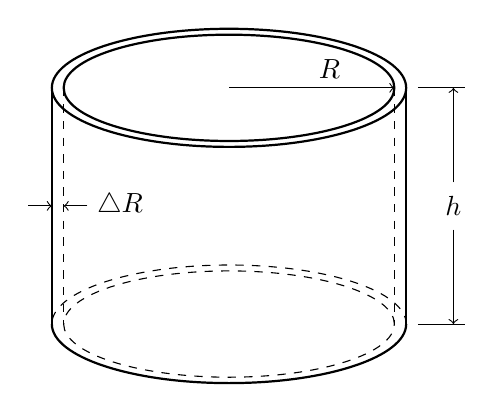
\begin{tikzpicture}[scale=1.5]
    \draw[thick,color=black] (1.5,2.0) arc (0:360:1.5 and 0.5); % Make the top ellipses
    \draw[thick,color=black] (1.4,2.0) arc (0:360:1.4 and 0.45);

    \draw[thick,color=black] ( 1.5,2.0) -- ( 1.5,0.0); % Mark the solid, straight sides
    \draw[thick,color=black] (-1.5,2.0) -- (-1.5,0.0);

    \draw[dashed,color=black] ( 1.4,2.0) -- ( 1.4,0.0); % Mark the inside sides
    \draw[dashed,color=black] (-1.4,2.0) -- (-1.4,0.0);

    \draw[thick,color=black]  (-1.5,0.0) arc (180:360:1.5 and 0.5); % Mark the bottom ellipses
    \draw[dashed,color=black] ( 1.5,0.0) arc (0:180:1.5 and 0.5);
    \draw[dashed,color=black] (1.4,0.0) arc (0:360:1.4 and 0.45);

    % Annotate the plot
    \draw[color=black,->] (0,2.0) -- (1.4,2.0) node[anchor=south] at (0.85,2) {$R$};
    \draw[color=black] (1.6,2) -- (2,2);
    \draw[color=black] (1.6,0) -- (2,0);
    \draw[color=black,->] (1.9,1.2) -- (1.9,2) node at (1.9,1) {$h$};
    \draw[color=black,->] (1.9,0.8) -- (1.9,0);
    \draw[color=black,->] (-1.7,1) -- (-1.5,1);
    \draw[color=black,->] (-1.2,1) -- (-1.4,1)  node[anchor=west] at (-1.2,1) {$\triangle R$};
  \end{tikzpicture}

  \vfill

\item Determine the value of the integral
  \begin{eqnarray*}
    \int^R_0 2\pi x \left( h-\frac{h}{R} x \right) ~ dx,
  \end{eqnarray*}
  where $h$ and $R$ are constants.
  \vfill


\end{problem}


\actTitle{Volumes of Revolution}
\begin{problem}
  \item Determine the formula for the volume of a cone.
      The base of the cone will have a radius of $R$ and the height will be $h$.
      The first step is to determine the formula for a line to revolve around the $y$-axis.
    \begin{subproblem}
      \item
        Make a sketch of the line that will be revolved around the $y$-axis.
        The base of the cone will be on the bottom, and the radius of the base of the resulting cone should be $R$.
        The height will be along the $y$-axis and should have a length of $h$.
        (Make the axes and clearly annotate the axes.)
        \vfill

      \item Make a sketch of the resulting solid obtained after
        revolving the line around the $y$-axis.
        \vfill

      \item Break up the domain ($x$) into pieces. Each piece of the domain will be used to make a rectangle
           from the $x$-axis to the function. The rectangle will be rotated around the $y$-axis to form a shell.
           Make a sketch of your function with one of the pieces revolved around the $y$-axis.
        \vfill

      \clearpage

      \item Determine the formula for the volume of one shell at $x_i$. Your answer should only be a function of $x_i$.
        \vfill

      \item Determine the formula for the Riemann sum representing an approximation of the volume.
        \vfill

      \item Take an appropriate limit of the Riemann sum and express the sum as an integral.
        \vfill

      \item Evaluate the integral to get the volume of the cone.
        \vfill

    \end{subproblem}

    \clearpage

    \item A cone is formed by rotating a straight line around the $y$-axis.
       The cone has a charge density, and the charge is a function of the radius, $r$,
       \begin{eqnarray*}
         \lambda_C(r) & = & \frac{2}{r^2+r+2} ~ \mathrm{C/m}^3
       \end{eqnarray*}
       The radius of the base of the cone is 0.3m, and the height of the cone is 0.4m.
       \begin{subproblem}
         \item
           Make a sketch of the line that will be revolved around the $y$-axis.
           The base of the cone will be on the bottom.
           The height will be along the $y$-axis.
           (Make an axis and clear mark the axes.)
           \vfill

         \item Make a sketch of the resulting solid obtained after
           revolving the line around the $y$ axis.
           \vfill

         \item Break up the domain ($x$) into pieces. Each piece of the domain will be used to make a rectangle
              from the $x$-axis to the function. The rectangle will be rotated around the $y$-axis to form a small cylinder.
              Make a sketch of your function with one of the pieces revolved around the axis.
           \vfill

         \clearpage

         \item Determine the formula for the volume of one small shell at $x_i$. Your answer should only be a function of $x_i$.
           \vfill

         \item Determine the formula for the charge of one small shell at $x_i$.
           \vfill

         \item Determine the formula for the Riemann sum representing an approximation of the volume.
           \vfill

         \item Take an appropriate limit of the Riemann sum and express the sum as an integral.
           \vfill

       \end{subproblem}
\end{problem}

\postClass

\begin{problem}
\item Briefly state two ideas from today's class.
  \begin{itemize}
  \item
  \item
  \end{itemize}
\item
  \begin{subproblem}
    \item
  \end{subproblem}
\end{problem}



%=========================================================================
% Start of Areas of Revolution
%=========================================================================
\preClass{Area of Revolution}

\begin{problem}
\item Determine the area of the sector of a circle shown below in
  terms of
  $\theta$ and $R$.
  %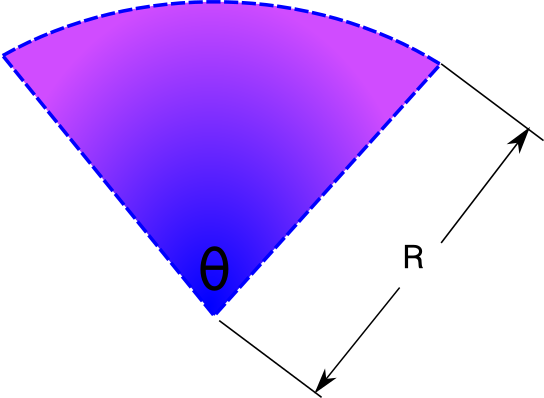
\includegraphics[width=12em]{ink/revolution/sector}

  \begin{tikzpicture}[scale=2.5,>={Latex[angle=45:5pt 2]}]
    \fill[left color=gray!50!black,right color=gray!50,middle color=gray!50,shading=axis,opacity=0.25] (0,0) -- (60:1) arc (60:120:1) -- (0,0);
    \draw[black,thick] (0,0) -- (60:1) arc (60:120:1) -- (0,0)
       node[anchor=south,shift={(0,0.2)}] {$\theta$} ;
    \draw[black] (0.05,0.0866) arc (60:120:.1);
    \begin{scope}[shift={(0.04,-0.025)}]
      \draw[black] (60:1) -- ++(-30:0.4);
      \draw[black] (0,0) -- ++(-30:0.4);
      \draw[black,<-] (-30:0.3) -- ++(60:0.3) node at ++(60:0.2) {$R$};
      \draw[black,->] (0.6,0.46) -- ++(60:0.3);
    \end{scope}

  \end{tikzpicture}


\item Determine the area of the slice of a sector shown below in terms of
  $\theta$, $L_1$, and $L_2$.
  %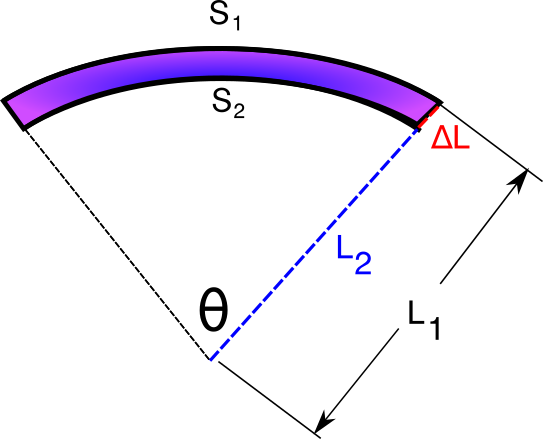
\includegraphics[width=12em]{ink/revolution/sectorDifference}

  \begin{tikzpicture}[scale=3.5,>={Latex[angle=45:5pt 2]}]
    \fill[left color=gray!50!black,right color=gray!50,middle color=gray!50,shading=axis,opacity=0.25]
       (60:1) arc (60:120:1) -- (120:0.85) arc (120:60:0.85) -- (60:1);
    %\fill[color=white] (0,0) -- (60:0.85) arc (60:120:0.85) -- (0,0);
    \draw[black,thick] (0,0) -- (60:1) arc (60:120:1) -- (0,0)
       node[anchor=south,shift={(0,0.2)}] {$\theta$} ;
    \draw[black,thick] (60:0.85) arc (60:120:0.85);
    \draw[black] (0.05,0.0866) arc (60:120:.1);
    \begin{scope}[rotate=-30,shift={(0.05,0)}]
      \draw[black] (0,1) -- ++(0.6,0);
      \draw[black] (0,0) -- ++(0.6,0);
      \draw[black,<-] (0.5,0) -- (0.5,0.3) node at ++(0,0.2) {$L_1$};
      \draw[black,->] (0.5,0.6) -- (0.5,1);
      \draw[black] (0,0.85) -- (0.15,0.85);
      \draw[black,<-] (0.1,0) -- (0.1,0.2) node at (0.1,0.3) {$L_2$};
      \draw[black,->] (0.1,0.5) -- (0.1,0.85);
      \node[font=\small] at (0.1,0.92) {$\triangle L$};
    \end{scope}
    %\node[anchor=north west,font=\small] at (60:0.45) {$L_2$};

    \node[black,anchor=south] at (0,1) {$S_1$};
    \node[black,anchor=north] at (0,0.85) {$S_2$};

  \end{tikzpicture}


\item Use the relationship $L_1 = L_2+\triangle L$ to express the area
  of the strip in terms of $\theta$, $\triangle L$, and  $L_2$.
  Expand and simplify the result.
  \label{problem:revol:area}
  \vfill
  \vfill

\item Substitute  $L_2\theta=S_2$  into the expression
  for the area in part \ref{problem:revol:area}.

  \vfill

\item Show that ${S_1-S_2}= \triangle L \theta$.

  \vfill


\item Substitute the expression found for $\triangle L \theta$ in the
  expression for the area. Simplify your result, and you should have a
  formula for the area of the strip only in terms of $S_1$, $S_2$, and
  $\triangle L$.

  \vfill

  \sideNote{Hint: $\triangle L^2\theta = \triangle L \cdot \triangle L \theta$}


\end{problem}

\actTitle{Area of Revolution}
\begin{problem}
  \item Determine the formula for the area of the side of a cone.
      The base of the cone will have a radius of $R$ and the height will be $h$.
      The first step is to determine the formula for a line to revolve around the $x$-axis.
  \begin{subproblem}
    \item Make a sketch of the line. (Make an axis and clearly mark the
      axes.)
      \vfill

    \item Make a sketch of the resulting cone obtained after
      revolving the line around the $x$-axis.
      \vfill

    \item Break up the domain ($x$) into pieces. Each piece of the domain will be used to make a small line segment.
         The line segment will be rotated around the $x$-axis to form a small frustum.
         Make a sketch of your function with one of the pieces revolved around the $x$-axis.
      \vfill

    \clearpage

    \item Determine the formula for the area of one small frustum at $x_i$. Your answer should only be a function of $x_i$.
      \vfill

    \item Determine the formula for the Riemann sum representing an approximation of the area.
      \vfill

    \item Take an appropriate limit of the Riemann sum and express the sum as an integral.
      \vfill

    \item Evaluate the integral to get the area of the side of a cone.
      \vfill



  \end{subproblem}
\end{problem}

\postClass

\begin{problem}
\item Briefly state two ideas from today's class.
  \begin{itemize}
  \item
  \item
  \end{itemize}
\item
  \begin{subproblem}
    \item
  \end{subproblem}
\end{problem}

\clearpage

\section{Flux through a surface}
The flux through a surface is defined to be the part of a vector field
that is normal to a surface mutliplied by the surface area. Before
discussing how to find the part of a vector that is normal to a
surface we will first look at surface area. In particular, we will
examine how to find the surface area that is formed by rotating a
curve around an axis.

\subsection{Areas of Revolution}
One way to form a surface is to take a curve and rotate it around some
axis. This process can be thought of as taking a string and
``twirling'' it around the axis, just like swinging a jump rope. For
example, one way to form a sphere is to take half of a circular
``hoop'' and spin it around an axis (see Figure
\ref{flux:figure:circle}) Another example is a cylinder which can be
formed by rotating a straight, horizontal line around an axis.

\begin{figure}[ht]
  \begin{center}
    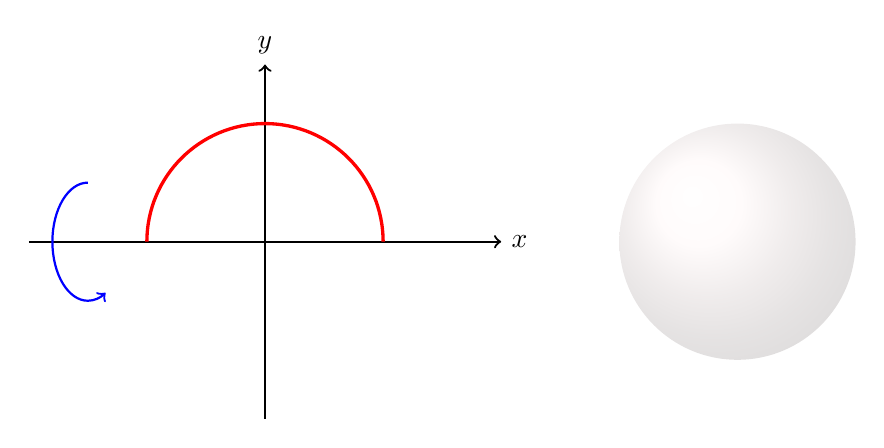
\begin{tikzpicture}[scale=1.5]
      \draw[thick,->] (-2,0) -- (2,0) node[anchor=west]  {$x$};
      \draw[thick,->] (0,-1.5) -- (0,1.5) node[anchor=south] {$y$};
      \draw[very thick,red] (1,0) arc (0:180:1);
      \draw[thick,blue,->] (-1.5,0.5) arc (90:300:0.3 and 0.5);
      \shade[ball color=red!10!white,opacity=0.20] (4,0) circle (1);
     \end{tikzpicture}

     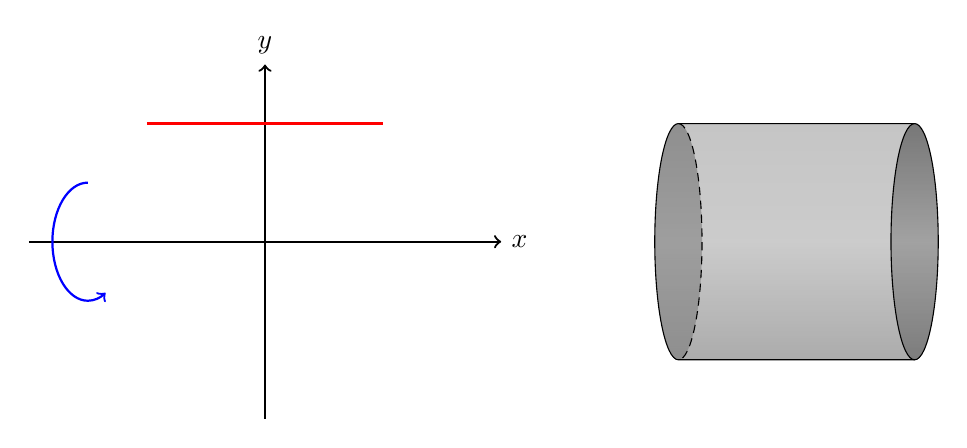
\begin{tikzpicture}[scale=1.5]
       \draw[thick,->] (-2,0) -- (2,0) node[anchor=west]  {$x$};
       \draw[thick,->] (0,-1.5) -- (0,1.5) node[anchor=south] {$y$};
       \draw[very thick,red] (-1,1) -- (1,1);
       \draw[thick,blue,->] (-1.5,0.5) arc (90:300:0.3 and 0.5);

       % Shade the bottom of the cylinder
       \fill[top color=gray!50!black,bottom color=gray!10,middle color=gray,
             shading=axis,opacity=0.25,shading angle=0] (3.5,0) circle (0.2 and 1);
       % Shade the outside of the cylinder
       \fill[left color=gray!30,right color=gray!90!black,middle color=gray!10,
             shading=axis,opacity=0.25,shading angle=0] (3.5,-1) -- (5.5,-1) arc (-90:90:0.2 and 1) -- (3.5,1) arc (90:270:0.2 and 1);
       % Shade the inside of the cylinder
       \fill[top color=gray!30!black,bottom color=gray!90!black,middle color=gray!50,
             shading=axis,opacity=0.25,shading angle=0] (5.5,0) circle (0.2 and 1);
       % Make an outline to make it really purty
       \draw (5.5,1) -- (3.5,1) arc (90:270:0.2 and 1) -- (5.5,-1);
       \draw (5.5,0) circle (0.2 and 1);
       \draw[densely dashed] (3.5,1) arc (90:-90:.2 and 1);
      \end{tikzpicture}

  \end{center}
  \caption{A half circle can be rotated around the $x$-axis to form a
    sphere. A straight, horizontal line can also be rotated around the
    $x$-axis to form a cylinder.}
  \label{flux:figure:circle}
\end{figure}

Other curves can be rotated around the axis, and the question is how
to find the resulting surface area given a formula for the curve.  The
basic idea to find the surface area of such a surface is to divide up
the original curve into small pieces, revolve each little piece around
the axis, and then add up the surface areas for all of the little
pieces.


\begin{figure}[ht]
%%>> \centerline{\psfig{file=notes/flux/fluxRiemann.eps,width=5in}}
\begin{center}
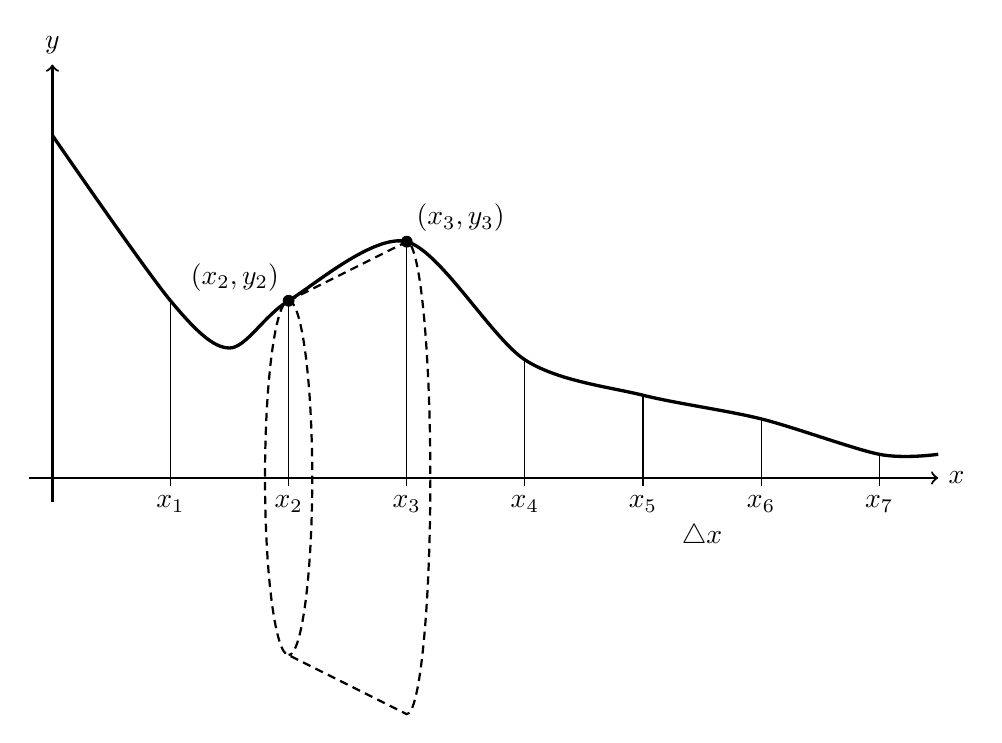
\begin{tikzpicture}[scale=1.5]
  \draw[thick,->] (-0.2,0) -- (7.5,0) node[anchor=west]  {$x$};
  \draw[thick,->] (0,-0.2) -- (0,3.5) node[anchor=south] {$y$};
   \draw [black, very thick] plot [smooth,tension=0.5] coordinates { % , tension=0.3
      (0,2.9) (1,1.5) (1.5, 1.1) (2,1.5) (3,2) (4,1) (5,0.7) (6,0.5) (7,0.2) (7.5,0.2)};

   \foreach \x in {1,2,...,7} {
      \draw (\x,2pt) -- (\x,-2pt) node[anchor = north] {$x_{\x}$};
    }

   \draw [black,thin] (0,0) -- (0,2.9);
   \draw [black,thin] (1,0) -- (1,1.5);
   \draw [black,thin] (2,0) -- (2,1.5);
   \draw [black,thin] (3,0) -- (3,2);
   \draw [black,thin] (4,0) -- (4,1);
   \draw [black,thin] (5,0) -- (5,0.7);
   \draw [black,thin] (6,0) -- (6,0.5);
   \draw [black,thin] (7,0) -- (7,0.2);

   \fill[black] (2,1.5) circle (0.05) node[anchor=south east] {$(x_2,y_2)$};
   \fill[black] (3,2) circle (0.05) node[anchor=south west] {$(x_3,y_3)$};
   \draw[black,thick,densely dashed] (2,1.5) -- (3,2) arc (90:-90:.2 and 2) -- (2,-1.5) arc (270:-90:0.2 and 1.5);
   \node at (5.5,-0.5) {$\triangle x$};
 \end{tikzpicture}
 \end{center}
\caption{The curve is divided up into pieces and each piece is
  revolved around the $x$-axis.}
\label{flux:figure:Riemann}
\end{figure}


For the general case, a curve given by $y=f(x)$\ is rotated around the
$x$-axis from $x=a$\ to $x=b$, and the resulting surface area will be
found.  The first step is to break up the curve into small pieces. In
order to take advantage of the fundamental theorem of calculus, the
\textbf{domain} will have to be divided up into small pieces first.
The domain, the values on the $x$-axis from $a$\ to $b$, is first
divided into small pieces of length $\triangle x$. Any segment along
the line starts at $x_n=a+n\triangle x$\ and ends at
$x_{n+1}=a+(n+1)\triangle x$ (see Figure \ref{flux:figure:Riemann}). (
The process of breaking the domain up into small pieces is called
``discretization''.)

\begin{figure}[ht]
%%>> \centerline{\psfig{file=notes/flux/fluxPieceDX.eps,height=3in}}
\begin{center}
  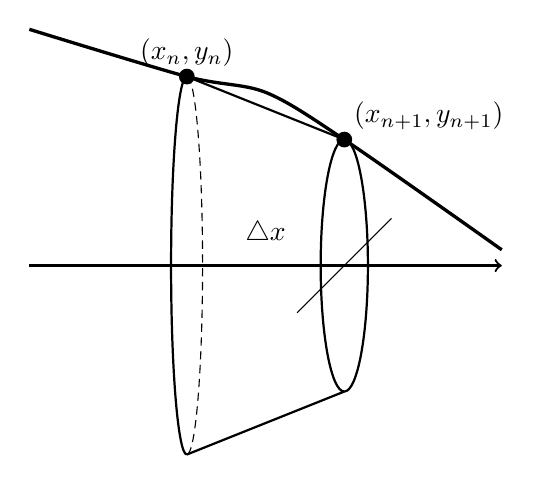
\begin{tikzpicture}[scale=2]
    \draw[thick,->] (1,0) -- (4,0);
     \draw [black, very thick] plot [smooth,tension=0.5] coordinates {
        (1,1.5) (2,1.2) (2.5,1.1) (3,0.8) (4,0.1)};

     %\draw [black,thin] (2,0) -- (2,1.2);
     %\draw [black,thin] (3,0) -- (3,0.8);
     \fill[black] (2,1.2) circle (0.05)  node [anchor=south] {$(x_n,y_n)$};
     \fill[black] (3,0.8) circle (0.05)  node [anchor=south west] {$(x_{n+1},y_{n+1})$};
     \draw[black,thick] (2,-1.2) -- (3,-0.8) arc (-90:270:.15 and 0.8);
     \draw[black,thick] (3, 0.8) -- (2, 1.2) arc (90:270:0.1 and 1.2);
     \draw[black,densely dashed] (2,1.2) arc (90:-90:0.1 and 1.2);
     \draw[black,thin] (3.3,.3) -- (2.7,-.3);
     \node at (2.5,0.2) {$\triangle x$};
   \end{tikzpicture}
\end{center}
\caption{The area of a line segment that is rotated around the
  $x$-axis is $2\pi\frac{y_{n+1}+y_n}{2}\triangle s$.}
\label{flux:figure:lineSegmentDX}
\end{figure}

Given a formula for a line we will find the area found by revolving
the line around the $x$-axis. Since the function changes according to
some variable, $x$, we will try to express the surface area of each
little piece that is found as a function of $x$\ and mutliplied by a
$\triangle x$. If we can do this, the sum can later be expressed as an
integral. An example of one of the little pieces can be seen in Figure
\ref{flux:figure:lineSegmentDX}.

\begin{figure}[tbh]
%%>> \centerline{\psfig{file=notes/flux/fluxPiece.eps,height=3in}}
\begin{center}
  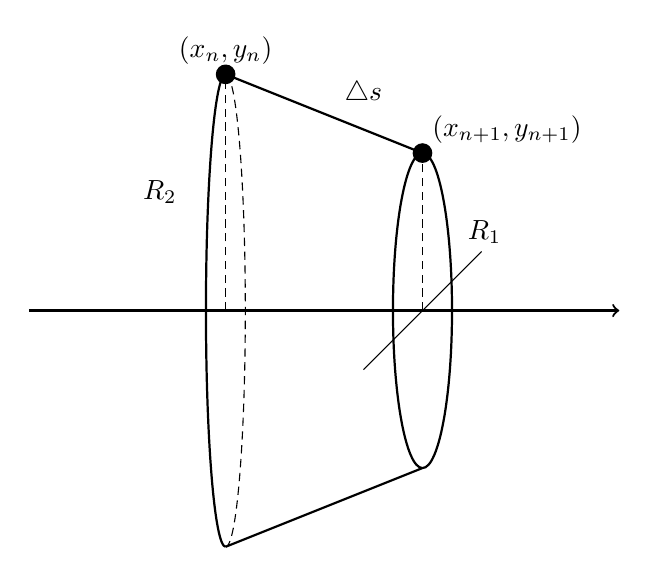
\begin{tikzpicture}[scale=2.5]
    \draw[thick,->] (1,0) -- (4,0);
     %\draw [black,thin] (2,0) -- (2,1.2);
     %\draw [black,thin] (3,0) -- (3,0.8);
     \fill[black] (2,1.2) circle (0.05)  node [anchor=south] {$(x_n,y_n)$};
     \fill[black] (3,0.8) circle (0.05)  node [anchor=south west] {$(x_{n+1},y_{n+1})$};
     \draw[black,thick] (2,-1.2) -- (3,-0.8) arc (-90:270:.15 and 0.8);
     \draw[black,thick] (3, 0.8) -- (2, 1.2) arc (90:270:0.1 and 1.2);
     \draw[black,densely dashed] (2,1.2) arc (90:-90:0.1 and 1.2);
     \draw[black,thin] (3.3,.3) -- (2.7,-.3);
     \node at (2.7,1.1) {$\triangle s$};
     \node[anchor=east] at (1.8,0.6) {$R_2$};
     \node[anchor=east] at (3.45,0.4) {$R_1$};
     \draw[black,densely dashed] (2,0) -- (2,1.2);
     \draw[black,densely dashed] (3,0) -- (3,0.8);
   \end{tikzpicture}
\end{center}
\caption{The area of a line segment that is rotated around the
  $x$-axis is $2\pi\frac{R_1+R_2}{2}\triangle s$.}
\label{flux:figure:lineSegment}
\end{figure}


Each little piece will be treated as a line segment of length
$\triangle s$\ that is rotated around the $x$-axis. If the distance
from the $x$-axis to the left side of the line segment is $R_1$ and
the distance from the $x$-axis to the right side of the line segment
is $R_2$, the area of the resulting surface is
$2\pi\frac{R_1+R_2}{2}\triangle s$. (See Figure
\ref{flux:figure:lineSegment}.)

Once the domain is subdivided, each straight line-segment from
$(x_n,y_n)$\ to $(x_{n+1},y_{n+1})$\ is revolved around the $x$-axis
(see Figure \ref{flux:figure:lineSegment}). The area of this one little
piece is
\begin{eqnarray*}
  2 \pi \frac{y_{n+1}+y_n}{2} \triangle s_n.
\end{eqnarray*}
The length, $\triangle s_n$, of the line segment (along the curve) can
be found through the use of the Pythagarean Theorem and is
\begin{eqnarray*}
  \triangle s_n & = & \sqrt{\lp x_{n+1}-x_n \rp^2 +
    \lp y_{n+1}-y_n \rp^2}.
\end{eqnarray*}
The notation can be simplified a bit, and the expression is factored
so that a $\triangle x_n$\ remains on the outside of the expression,
\begin{eqnarray*}
\triangle s_n  & = & \sqrt{ \triangle x_n^2 +  \triangle y_n^2}, \\
  & = & \sqrt{ 1 +  \lp \frac{\triangle y_n}{\triangle x_n} \rp^2}
  ~~ \triangle x_n.
\end{eqnarray*}
The $\triangle x_n$\ was factored out so that the whole expression can
later be written as a Riemann sum varying over the $x$\ values.

An approximation of the total surface area from $x=a$\ to $x=b$\ is
found by adding up all of the surface areas of the little pieces
together,
\begin{eqnarray}
  \sum^{N-1}_{n=0} 2 \pi \frac{y_{n+1}+y_n}{2}\triangle s_n & = &
  \sum^{N-1}_{n=0} 2 \pi \frac{y_{n+1}+y_n}{2}
  \sqrt{ 1 +  \lp \frac{\triangle y_n}{\triangle x_n} \rp^2} ~ \triangle x_n.
  \label{flux:eqn:riemann}
\end{eqnarray}
The $y$\ values are found by using the value of the function at the
points in its domain, $y_n=f(x_n)$. As the length of the line segments
get closer to zero the Riemann sum approachs an integral,
\begin{eqnarray*}
  \int^b_a 2 \pi f(x) \sqrt{1+\lp f'(x)\rp^2} ~ dx.
\end{eqnarray*}




\subsection{Area of a Sphere}
As an example, the surface area of a sphere of radius $R$\ is
found. A semi-circle, $f(x)=\sqrt{R^2-x^2}$, is rotated around the
$x$-axis. The area is given by the integral
\begin{eqnarray*}
  \int^R_{-R} 2 \pi \sqrt{R^2-x^2} \sqrt{1 + \lp
    \frac{-x}{\sqrt{R^2-x^2}} \rp^2 } ~ dx
    & = & \int^R_{-R} 2 \pi \sqrt{R^2-x^2} \sqrt{1 +
      \frac{x^2}{R^2-x^2}} ~ dx, \\
    & = & \int^R_{-R} 2 \pi \sqrt{R^2-x^2} \sqrt{
      \frac{R^2}{R^2-x^2}} ~ dx, \\
    & = & \int^R_{-R} 2 \pi R ~ dx, \\
    & = & 4 \pi R^2.
\end{eqnarray*}


\subsection{Flux Through a Surface From A Point Charge}
If a point charge is located at the origin the magnitude of the
electic field at a point, $(x,y)$, can be found using Coulomb's Law,
\begin{eqnarray*}
  |\vec{E}| & = & \frac{k\hat{q}}{x^2+y^2},
\end{eqnarray*}
where $\hat{q}$\  is the total charge  of the particle. The field will
be  pointing radially away   from the origin   (or inwards if it  is a
negative charge).  To  find the  flux through  a surface  two examples
will be examined. The first is the specific case of the flux through a
cylinder, and the second situation examined is the general case of the
flux through a surface.

For negative $x$\ values the vectors for the electric field point to
the left, and for positive $x$\ values the vectors for the electric
field point to the right. The result is that the process of finding
the components of the vectors is different for negative $x$\ values
than for positive $x$\ values. We will concentrate on finding the flux
for positive $x$\ values and leave the process of finding the flux for
negative values as an exercise for the reader. (The formulas for the
flux for the negative $x$\ values is the same except that a negative
sign in front of the resulting flux is required.)

\subsection{Flux Through A Cylinder}
A straight, horizontal line that is a distance $R$\ above the $x$-axis
can be rotated around the $x$-axis to define the surface of a cylinder
whose radius is $R$. It is assumed that the line is located in the
first quadrant. To find the flux through a cylinder of radius $R$\ and
length $L$\ from a point charge at the origin, a straight, horizontal
line is divided into small pieces, each small piece is rotated around
the $x$-axis, and the flux is calculated through the resulting area
(see Figure \ref{flux:figure:lineSegmentFlux}). The total flux is
found by adding the contribution of each of the line-segments.

\begin{figure}[ht]
%%>> \centerline{\psfig{file=notes/flux/fluxCylinder.eps,height=5in}}
\begin{center}
  \begin{tikzpicture}[scale=1.5,>={Latex[angle=45:5pt 2]}]
    \draw[thick,->] (-0.1,0) -- (4,0) node[anchor=west] {$x$};
    \draw[thick,->] (0,-2) -- (0,2) node[anchor=south] {$y$};
    \fill[black] (0,0) circle (0.1);
    \draw[densely dotted,black] (0,0) -- (3,1.5) -- (3,0);
    \draw[line width=1mm,blue] (2.7,1.5) -- (3.3,1.5);
    \draw[line width=1mm,black,tips=proper,->] (3,1.5) -- (4,2) node[anchor=west] {$\vec{E}$};
    \draw[densely dotted,black] (3,0) -- (3,1.5) node [shift={(0,-1)},anchor=west] {$R$};
    \draw[black] (0.5,0.25) arc (45:90:0.7) node [shift={(0.25,-0.12)},anchor=south west] {$\phi$};
    \node[anchor=north] at (1.5,0) {$x$};
    \node[anchor=north east] at (0,0) {$q$};
   \end{tikzpicture}
 \end{center}

 \begin{center}
   \begin{tikzpicture}[scale=1.5,>={Latex[angle=45:5pt 2]}]
     \fill[left color=gray!70,right color=gray!50,middle color=gray!02,shading=axis,opacity=0.05,shading angle=0,fill opacity=0.05] (2.7,1.5) -- (3.3,1.5) arc (90:270:0.2 and 1.5) -- (2.7,-1.5) arc (270:90:0.2 and 1.5);
     \draw[black] (2.7,1.5) -- (3.3,1.5) arc (90:270:0.2 and 1.5) -- (2.7,-1.5) arc (270:90:0.2 and 1.5);
     \draw[thick,->] (-0.1,0) -- (4,0) node[anchor=west] {$x$};
     \draw[thick,->] (0,-2) -- (0,2) node[anchor=south] {$y$};
     \fill[black] (0,0) circle (0.1);
     \draw[densely dotted,black] (0,0) -- (3, 1.5) -- (3,0);
     \draw[densely dotted,black] (0,0) -- (3,-1.5) -- (3,0);
     \node[anchor=north east] at (1.5,-0.75) {$\sqrt{x^2+R^2}$};
     \draw[line width=1mm,blue] (2.7,1.5) -- (3.3,1.5);
     \draw[line width=1mm,black,tips=proper,->] (3,1.5) -- (4,2) node[anchor=west] {$\vec{E}$};
     \draw[line width=1mm,black,tips=proper,->] (3,1.5) -- (3,2) node[anchor=east] {$\vec{n}$};
     \draw[black] (3,1.7) arc (90:45:0.3) node [shift={(-0.08,0.02)},anchor=south west] {$\phi$};
     \draw[densely dotted,black] (3,2) -- (4,2);
     \draw[black] (0.5,0.25) arc (45:90:0.7) node [shift={(0.25,-0.12)},anchor=south west] {$\phi$};
     \node[anchor=north] at (1.5,0) {$x$};
     \node[anchor=north east] at (0,0) {$q$};
     \fill[left color=gray!10!gray!30,right color=gray!10!gray!30,middle color=gray!5,shading=axis,shading angle=0,fill opacity=0.05] (2.7,1.5) -- (3.3,1.5) arc (90:-90:0.2 and 1.5) -- (2.7,-1.5) arc (-90:90:0.2 and 1.5);
     \draw[black]  (2.7,1.5) -- (3.3,1.5) arc (90:-90:0.2 and 1.5) -- (2.7,-1.5) arc (-90:90:0.2 and 1.5);
     %\draw[densely dotted,black] (3,0) -- (3,1.5) node [shift={(0,-1)},anchor=west] {$R$};
    \end{tikzpicture}
  \end{center}

\caption{The flux through an area is defined to be the magnitude of
  the vector normal to the surface multiplied by the surface area.}
\label{flux:figure:lineSegmentFlux}
\end{figure}

The area of one of the small ``hoops'' is $2\pi R \triangle x$ (here
$f(x)=R$, and $f'(x)=0$), and the flux is $|\vec{E}|\cos(\phi) 2\pi R
\triangle x$. The total flux is found by adding up the flux through
each piece:
\begin{eqnarray*}
  \sum^{N-1}_{n=0} |\vec{E}|\cos(\phi_n) 2\pi R \triangle x_n & = &
  \sum^{N-1}_{n=0} \frac{k\hat{q}}{x_n^2+R^2} \cos(\phi)
      2\pi R \triangle x_n.\\
\end{eqnarray*}
Assuming the line lies in the first quadrant, the cosine of $\phi$\ is
$\frac{R}{\sqrt{x_n^2+R^2}}$, and the resulting flux is
\begin{eqnarray*}
\sum^{N-1}_{n=0} \lp \frac{k\hat{q}}{x_n^2+R^2} \cdot
                     \frac{R}{\sqrt{x_n^2+R^2}}
      2\pi R \rp ~ \triangle x_n
  & = & \sum^{N-1}_{n=0} \lp \frac{k\hat{q}}{\lp x_n^2+R^2 \rp^{3/2}}
      2\pi R^2 \rp ~ \triangle x_n.
\end{eqnarray*}
As the length of the line-segments approaches zero the Riemann sum
approaches an integral,
\begin{eqnarray*}
  \int^L_{0} \frac{k\hat{q}}{\lp{x^2+R^2}\rp^{\frac{3}{2}}}
      2\pi R^2 ~dx.
\end{eqnarray*}

For a line segment in the second quadrant, the cosine of $\phi$\ has
the opposite sign, and the resulting integral appears to be the same
only with a negative sign in front of it.


\subsection{Flux Through A Surface of Revolution}
Finding the flux through a cylinder is made easier because the normal
to the line segment is always straight up (in the $\vec{\jmath}$\
direction). In the general case, however, the curve that is being
rotated is not necessarily a horizontal line, and the normal to the
surface can be more difficult to find. We will concentrate on finding
the portion of the electric field that is perpindicular to a straight
line-segment. Once this is found, a Riemann sum for the flux can be
found for the general problem.

\begin{figure}[ht]
  \begin{center}
    \begin{tikzpicture}[scale=1.5,>={Latex[angle=45:5pt 2]}]
      \draw[thick,->] (-0.2,0) -- (4,0) node[anchor=west] {$x$};
      \draw[thick,->] (0,-0.2) -- (0,4) node[anchor=south] {$y$};
      \fill[black] (0,0) circle (0.1);
      %\draw [black, very thick] plot [smooth,tension=0.5] coordinates { % , tension=0.3
      %   (0,2.9) (1,1.5) (1.5, 1.1) (2,1.5) (3,2) (4,1) (5,0.7) (6,0.5) (7,0.2) (7.5,0.2)};
      \draw[line width=1mm,black] (-0.2,1.5) .. controls (0.5,1.6) .. (1,2) .. controls (2,3.2) .. (3.5,4) node[shift={(-0.2,0)},anchor=south] {$f$};
      \draw[thick,->,black] (1,2) -- (0.4,2.8) node[anchor=south] {$\vec{n}$};
      \draw[thick,->,black] (1,2) -- (2,4) node[anchor=south] {$\vec{E}$};
      \draw[black] (1.2,2.4) arc (45:130:0.4) node[shift={(0.3,0)},anchor=south west] {$\theta$};

      \draw[very thick,green] (0,0) -- (1,2) -- (1,0) -- (0,0);
      \node[anchor=west,green] at (1,1) {$f(x)$};
      \draw[green] (0.2,0) arc (0:60:0.2) node[shift={(0.4,0)},green] {$\phi$};
      \draw[green] (1.8,2) arc (0:60:0.8) node[shift={(0.8,-0.5)},green] {$\phi$};
      \node[black,anchor=north] at (1,0) {$x$};

      \draw[thick,blue] (1,2) -- (3,2) -- (3,3.6) -- (1,2);
      \draw[blue] (1.2,2) arc (0:45:0.2) node[shift={(0.4,0)},blue] {$\psi$};
      \node[anchor=west,blue] at (3,2.8) {$f'(x)$};
      \node[anchor=north,blue] at (2,2) {$1$};

      \fill[black] (0,0) circle (0.1);
      \node[anchor=south east] at (0,0) {$q$};
      \node[anchor=south] at (3.5,0.7) {$\theta+\phi-\psi=\frac{\pi}{2}$};

     \end{tikzpicture}
   \end{center}
\caption{The component of a vector perpindicular to a surface is the
  length of the vector multiplied by the cosine of the angle between
  the vector and the normal to the surface.}
\label{flux:figure:lineSegmentGeneralFlux}
\end{figure}

First the component of the electric field that is normal to a
line-segment is found (see Figure
\ref{flux:figure:lineSegmentGeneralFlux}). (Again, it is assumed that
the line segment is in the first quadrant.) The component of the
electric field normal to a line-segment is the length of the vector
due to the electric field mutliplied by the cosine of the angle
between a vector perpindicular to the line and the vector from the
electric field. If the angle between the normal and a horizontal line
is $\psi$\ and the angle between the electric field and a horizontal
line is $\phi$, then the angle between the normal and the electric
field is $\frac{\pi}{2}+\psi-\phi$.

The cosine of $\frac{\pi}{2}+\psi-\phi$\ can be found by looking at
each separate angle:
\begin{eqnarray*}
  \cos(\frac{\pi}{2} + \psi-\phi) & = & -\sin(\psi-\phi), \\
  & = & \cos(\psi)\sin(\phi) - \sin(\psi)\cos(\phi).
\end{eqnarray*}
Since the point charge is located at the origin, the electric field is
pointing in a radial direction,
\begin{eqnarray}
  \label{flux:eqn:edirection}
  \cos(\phi) & = & \frac{x}{\sqrt{x^2+y^2}}, \\
  \sin(\phi) & = & \frac{y}{\sqrt{x^2+y^2}}. \nonumber
\end{eqnarray}
To handle the angle for the normal, some information must be known
about the function. The slope of the tangent line is given by the
derivative of the function, and the normal is the vector perpindular
to the tangent line (see Figure
\ref{flux:figure:lineSegmentGeneralFlux}):
\begin{eqnarray}
  \label{flux:eqn:fdirection}
  \cos(\psi) & = & \frac{1}{\sqrt{1+(f'(x))^2}}, \\
  \sin(\psi) & = & \frac{f'(x)}{\sqrt{1+(f'(x))^2}}. \nonumber
\end{eqnarray}

The component of the electric field that is normal to the line segment
is
\begin{eqnarray*}
  |\vec{E}| \cos(\frac{\pi}{2} + \psi-\phi) & = &
       \frac{k\hat{q}}{x^2+y^2}
  \lp \cos(\psi)\sin(\phi) - \sin(\psi)\cos(\phi) \rp,  \\
\end{eqnarray*}
which can be expanded using equations (\ref{flux:eqn:edirection}) and
(\ref{flux:eqn:fdirection}),
\begin{eqnarray*}
  \lefteqn{ \frac{k\hat{q}}{x^2+y^2}
       \lp \cos(\psi)\sin(\phi) - \sin(\psi)\cos(\phi) \rp  ~ = } &&  \\
     & &   \frac{k\hat{q}}{x^2+f^2(x)}
     \lp \frac{f(x)}{\sqrt{x^2+f^2(x)}} \cdot
     \frac{1}{\sqrt{1+\lp f'(x) \rp^2}} -
     \frac{x}{\sqrt{x^2+f^2(x)}} \cdot
     \frac{f'(x)}{\sqrt{1+\lp f'(x) \rp^2}} \rp.
\end{eqnarray*}
If the line segment is rotated around the $x$-axis the resulting flux
is given by
\begin{eqnarray*}
  \lefteqn{|\vec{E}| \cos(\frac{\pi}{2}+\psi-\phi)
    2\pi \frac{f(x_{n+1})+f(x_n)}{2}
    \sqrt{1+ \lp f'(x_n) \rp^2}  } \\
  & = & \frac{k\hat{q}}{x_n^2+y_n^2}
  \lp \cos(\psi)\sin(\phi) - \sin(\psi)\cos(\phi) \rp
     2\pi \frac{f(x_{n+1})+f(x_n)}{2} \sqrt{1+ \lp f'(x_n) \rp^2} ~
     \triangle x_n.  \\
\end{eqnarray*}
After substituting from equations (\ref{flux:eqn:edirection}) and
(\ref{flux:eqn:fdirection}), the flux for one piece can be expressed
as
\begin{eqnarray*}
  \frac{k\hat{q}}{\lp x_n^2+f^2(x_n)\rp^{3/2} }
  \lp f(x_n) - x_n f'(x_n) \rp 2 \pi \frac{f(x_{n+1})+f(x_n)}{2} ~
  \triangle x_n.
\end{eqnarray*}

The total flux can be approximated by adding up the fluxes through
each small piece to give
\begin{eqnarray*}
  \sum_{n=0}^N \lp \frac{k\hat{q}}{\lp x_n^2+f^2(x_n)\rp^{3/2} }
  \lp f(x_n) - x_n f'(x_n) \rp 2 \pi \frac{f(x_{n+1})+f(x_n)}{2} \rp
  ~ \triangle x_n.
\end{eqnarray*}
As the length of the line segments goes to zero, the Riemann sum
approachs the integral
\begin{eqnarray*}
  k\hat{q}2\pi \int^b_a f(x)\frac{f(x)-xf'(x)}{\lp x^2+f^2(x) \rp^{3/2}}
     ~ dx & = &
     k\hat{q}2\pi \int^b_a \frac{f^2(x)-xf(x)f'(x)}{\lp x^2+f^2(x)
       \rp^{3/2}} ~ dx.
\end{eqnarray*}
An $x^3$\ can be factored from the denomintor to yield
\begin{eqnarray*}
  k\hat{q}2\pi \int^b_a \frac{f^2(x)-xf(x)f'(x)}{x^3 \lp
    1+\lp \frac{f(x)}{x} \rp^2 \rp^{3/2}} ~ dx,
\end{eqnarray*}
and the $x^3$\ can be factored into the numerator which gives
\begin{eqnarray*}
  k\hat{q}2\pi \int^b_a \frac{x^{-3}f^2(x)-x^{-2}f(x)f'(x)}{\lp
    1+\lp \frac{f(x)}{x} \rp^2 \rp^{3/2}} ~ dx.
\end{eqnarray*}
The resulting integral can be found by using $u$-substition, where
$u=\lp \frac{f(x)}{x} \rp^2$ giving
\begin{eqnarray*}
    \frac{k\hat{q}2\pi}{\sqrt{1+\lp \frac{f(x)}{x} \rp^2 }}
     \Bigg|^b_a
     & = & \frac{k\hat{q}2\pi x}{\sqrt{x^2 + f(x)^2}}
     \Bigg|^b_a.
\end{eqnarray*}



%=========================================================================
% Start of flux through a surface
%=========================================================================
\preClass{Flux Through A Surface}

\begin{problem}
\item An electric field is given by
\begin{eqnarray*}
  \vec{E} & = & 3 \vec{k}.
\end{eqnarray*}
A surface is defined by the square with corners at $P_1(0,0,1)$, $P_2(2,0,1)$, $P_3(2,2,1)$, and $P_4(0,2,1)$.
\begin{subproblem}
  \item Make a sketch of the square in a 3D coordinate system. Make sure to include the axes and label the axes.
    \vfill
  \item Determine the flux through the square.
    \vfill
  \item Determine the flux through the square if the electric field is $\vec{E} = 2\vec{\imath} + 3\vec{k}$ instead.
    \vfill
\end{subproblem}
\end{problem}


\actTitle{Flux Through A Surface}


\begin{problem}
\item The flux through a cylinder for a point charge at the origin is found.
A horizontal line will be rotated around the $x$-axis to form a cylinder.
  \begin{subproblem}
    \item Make a sketch of the situation. First draw and label the $x$ and $y$-axes.
    Place a point charge at the origin.
    Finally, draw the function that will result in a cylinder of radius $R$ and length $L$ when it is rotated aroun the $x$ axis.
    The left end of the cylinder should be at $x=0$.
    \vfill

    \item Redraw your sketch above. Divide up the domain, $x$, into small pieces.
    Indicate a small piece that will be rotated around the $x$-axis at some $x_i$.
    Sketch the electric field that will go through the piece.
    Sketch the normal vector to the small piece and label the angle, $\theta$, between the normal and the electric field.
    \vfill

    \item  Determine the magnitude of the  electric field at the small piece and determine the scalar component in the direction of the normal.
    \vfill

    \clearpage

    \item Determine the flux through the thin strip after it has been rotated around the $x$-axis.
      \vfill

    \item Determine the approximation of the total flux by adding up all of the fluxes for each small strip.
      \vfill

    \item Take the appropriate limit and express the flux as an integral.
      \vfill

    \item Determine the total flux through the cylinder.
      \vfill

    \clearpage

    \item What happens to the flux as $L$ gets very large?
      \vspace{6em}

    \item What is the flux through a cylinder with length $2L$ and radius $R$ centered at the origin? What happens to the value of the flux as $L$ gets very large?
      \vfill

  \end{subproblem}
\end{problem}


\postClass

\begin{problem}
\item Briefly state two ideas from today's class.
  \begin{itemize}
  \item
  \item
  \end{itemize}
\item
  \begin{subproblem}
    \item
  \end{subproblem}
\end{problem}


%=========================================================================
% Start of partial fractions
%=========================================================================
\preClass{Rational Functions}

\begin{problem}
\item Express each function below as a single fraction. That is bring
  the two parts together over a common denominator and simplify the
  result.
  \begin{subproblem}
  \item $\frac{1}{3} + \frac{1}{4}$
    \vfill
  \item $\frac{1}{x+3} + \frac{3}{x-2}$
    \vfill
  \item $\frac{1}{x+3} + \frac{4}{x-3}$
    \vfill
  \end{subproblem}
\end{problem}


\actTitle{Partial Fractions}
\begin{problem}
\item Determine the common denominator for each of the expressions below.
  \begin{subproblem}
    \item $\frac{1}{x} + \frac{1}{x-3}$ \\
      Common Denominator: \framebox(250,50){~}
      \vfill
    \item $\frac{8}{x+7} + \frac{20}{x+5}$ \\
      Common Denominator: \framebox(250,50){~}
      \vfill
    \item $\frac{8,250}{x+7} + \frac{x}{x+5}$ \\
      Common Denominator: \framebox(250,50){~}
      \vfill
  \end{subproblem}

  \clearpage

\item For each of the following functions write the general form of
  the partial fraction expansion. The first one is completed as an
  example.
  \begin{subproblem}
    \item $\frac{2x+1}{x^2+2x-8}$ \\
      General Form: \framebox(250,50){$\frac{A}{x+4} + \frac{B}{x-2}$}
    \item $\frac{8x+1}{x^2-x-12}$ \\
      General Form: \framebox(250,50){~}
      \vfill
    \item $\frac{5x-10}{x^2-16}$ \\
      General Form: \framebox(250,50){~}
      \vfill
    \item $\frac{4x+2}{x^2-5x}$ \\
      General Form: \framebox(250,50){~}
      \vfill
  \end{subproblem}

  \clearpage

  \item For each of the functions on the previous page determine the values of the constants.
    The first one is completed as an example.
    \begin{subproblem}
      \item $\frac{2x+1}{x^2+2x-8}$ \\
      \begin{tabular}{ll}
        General Form: & $\frac{2x+1}{x^2+2x-8}=\frac{A}{x+4} + \frac{B}{x-2}$ \\ [10pt]
        Multiply by the common denominator:  & $\frac{(2x+1)(x-2)(x+4)}{x^2+2x-8}=\frac{A(x+4)(x-2)}{x+4} + \frac{B(x+4)(x-2)}{x-2}$ \\ [10pt]
        Simplify: & $(2x+1)=A(x-2) + B(x+4)$ \\ [10pt]
        Let $x=2$: & $2\cdot 2 + 1 = A(0) + B(2+4) \rightarrow B=\frac{5}{6}$. \\ [10pt]
        Let $x=-4$: & $(2\cdot (-4) + 1) = A(-4-2) + B(-4+4) \rightarrow A=\frac{-7}{-6}$. \\ [10pt]
        Result: & $\frac{2x+1}{x^2+2x-8}=\frac{7/6}{x+4} + \frac{5/6}{x-2}$
      \end{tabular}
      \item $\frac{8x+1}{x^2-x-12}$ \\
        \vfill

        \clearpage
      \item $\frac{5x-10}{x^2-16}$ \\
        \vfill
      \item $\frac{4x+2}{x^2-5x}$ \\
        \vfill
    \end{subproblem}


\end{problem}

\postClass

\begin{problem}
\item Briefly state two ideas from today's class.
  \begin{itemize}
  \item
  \item
  \end{itemize}
\item
  \begin{subproblem}
    \item
  \end{subproblem}
\end{problem}


\preClass{Rational Functions}

\begin{problem}
\item Express each function below as a single fraction. That is bring
  the two parts together over a common denominator and simplify the
  result.
  \begin{subproblem}
  \item ${\displaystyle \frac{1}{x+2} + \frac{3}{(x+2)^2}}$
    \vfill
  \item ${\displaystyle \frac{1}{x+3} + \frac{2}{(x+3)^2}}$
    \vfill
  \item ${\displaystyle \frac{1}{x} + \frac{1}{x^2} + \frac{1}{x^3}}$
    \vfill
  \end{subproblem}
\end{problem}

\actTitle{Partial Fractions}
\begin{problem}
\item Determine the common denominator for each of the expressions below.
  \begin{subproblem}
    \item ${\displaystyle \frac{1}{x-3} + \frac{1}{x^2-6x+9}}$ \\
      Common Denominator: \framebox(250,50){~}
      \vfill
    \item ${\displaystyle \frac{2}{x+2} + \frac{4}{x^2+x+1}}$ \\
      Common Denominator: \framebox(250,50){~}
      \vfill
    \item ${\displaystyle \frac{3}{x+2} + \frac{x}{x^2+x+1}}$ \\
      Common Denominator: \framebox(250,50){~}
      \vfill
  \end{subproblem}

  \clearpage

\item For each of the following functions write the general form of
  the partial fraction expansion.
  \begin{subproblem}
    \item ${\displaystyle \frac{2x+1}{x^2-6x+9}}$ \\
      General Form: \framebox(250,50){~}
      \vfill
    \item ${\displaystyle \frac{2x^2+6x+10}{x^3+3x^2+3x+2}}$ \\
      General Form: \framebox(250,50){~}
      \vfill
    \item ${\displaystyle \frac{3x^2+4x+2}{x^3+3x^2+3x+2}}$ \\
      General Form: \framebox(250,50){~}
      \vfill
  \end{subproblem}

\clearpage

\item For each of the following antiderivatives write the general form of
the partial fraction expansion, and then solve for the unknown constants.
Finally solve for the general anti-derivative if you have time.
\begin{subproblem}
  \item ${\displaystyle \int \frac{2x+1}{x^2-6x+9} ~ dx}$
    \vfill
  \item ${\displaystyle \int \frac{2x^2+6x+10}{x^3+3x^2+3x+2}~ dx}$
    \vfill
    \clearpage
  \item ${\displaystyle \int \frac{3x^2+4x+2}{x^3+3x^2+3x+2} ~ dx}$
    \vfill
\end{subproblem}

\end{problem}


\postClass

\begin{problem}
\item Briefly state two ideas from today's class.
  \begin{itemize}
  \item
  \item
  \end{itemize}
\item
  \begin{subproblem}
    \item
  \end{subproblem}
\end{problem}


\preClass{Rational Functions}

\begin{problem}
\item For each of the quadratic functions below complete the square to
  express each function in the form
  \begin{eqnarray*}
    f(x) & = & A(x-B)^2 + C.
  \end{eqnarray*}
  \begin{subproblem}
  \item $x^2 - 2x + 2$
    \vfill
  \item $x^2 - 6x + 12$
    \vfill
  \item $2x^2 - 4x + 6$
    \vfill
  \end{subproblem}
\end{problem}

\actTitle{Partial Fractions}
\begin{problem}
\item For each integral below complete the square on the denominator
  and then use $u$-substitution to determine the integral.
  \begin{subproblem}
    \item ${\displaystyle \int}\frac{1}{x^2 - 2x + 2}~dx$ \\
      \vfill
    \item ${\displaystyle\int}\frac{2}{x^2 - 6x + 12}~dx$ \\
      \vfill
    \item ${\displaystyle\int}\frac{1}{x^2 + 8x + 26}~dx$ \\
      \vfill
  \end{subproblem}

  \clearpage

\item Determine the value of the integral
  \begin{eqnarray*}
    \int \frac{1}{x^3+x^2+3\,x-5} ~ dx
  \end{eqnarray*}

  \vfill

\end{problem}


\postClass

\begin{problem}
\item Briefly state two ideas from today's class.
  \begin{itemize}
  \item
  \item
  \end{itemize}
\item
  \begin{subproblem}
    \item
  \end{subproblem}
\end{problem}





%%% Local Variables:
%%% mode: latex
%%% TeX-master: t
%%% End:
